\documentclass[11pt]{article}

\usepackage[paperwidth=16cm,paperheight=9cm,margin=0cm]{geometry}
\usepackage[T1]{fontenc}
\usepackage{lmodern}
\usepackage{tikz}
\usepackage{graphicx}
\usepackage{xcolor}
\usepackage{listings}
\usepackage{booktabs}
\usepackage{array}
\usetikzlibrary{arrows.meta,positioning,calc,shapes.geometric}

\pagestyle{empty}
\setlength{\parindent}{0pt}
\renewcommand{\familydefault}{\sfdefault}
\hyphenpenalty=10000
\exhyphenpenalty=10000

\definecolor{Paper}{HTML}{FFF7ED}
\definecolor{PaperSoft}{HTML}{FFFDF8}
\definecolor{Ink}{HTML}{221714}
\definecolor{Muted}{HTML}{6B5A50}
\definecolor{Line}{HTML}{E7CDB7}
\definecolor{Coral}{HTML}{EF5B42}
\definecolor{Blue}{HTML}{2F8CEB}
\definecolor{Gold}{HTML}{F5B842}
\definecolor{Green}{HTML}{2E9C6D}
\definecolor{Red}{HTML}{C44536}
\definecolor{Navy}{HTML}{10233F}

\pagecolor{Paper}
\color{Ink}

\newcounter{slideno}

\newenvironment{slideframe}[1]{%
  \ifnum\value{slideno}>0\newpage\fi
  \stepcounter{slideno}
  \thispagestyle{empty}
  \begin{tikzpicture}[remember picture,overlay]
    \fill[Coral] ([xshift=0.65cm,yshift=-0.55cm]current page.north west) circle (0.08cm);
    \fill[Gold] ([xshift=0.90cm,yshift=-0.55cm]current page.north west) circle (0.055cm);
    \node[anchor=south east,font=\scriptsize\bfseries,text=Muted] at ([xshift=-0.55cm,yshift=0.34cm]current page.south east) {Fleeting Circus \thepage};
  \end{tikzpicture}
  \par\vspace*{1.42cm}
  \hspace*{0.8cm}
  \begin{minipage}{14.35cm}
    {\fontsize{21}{25}\selectfont\bfseries #1\par}
    \vspace{0.36cm}
}{%
  \end{minipage}
}

\newcommand{\titletext}[1]{{\fontsize{28}{32}\selectfont\bfseries #1\par}}
\newcommand{\subtitletext}[1]{{\fontsize{14}{18}\selectfont\color{Muted}#1\par}}
\newcommand{\labeltext}[1]{{\fontsize{8}{10}\selectfont\bfseries\color{Coral}\MakeUppercase{#1}\par}}
\newcommand{\plainitem}[1]{\par\noindent\begin{tikzpicture}[baseline=-0.5ex]\fill[Coral] (0,0) circle (0.055cm);\end{tikzpicture}\hspace{0.35em}{#1}}
\newcommand{\pill}[2]{\tikz[baseline=-0.7ex]\node[rounded corners=5pt,draw=#1!55,fill=#1!12,inner xsep=6pt,inner ysep=3pt,font=\scriptsize\bfseries] {#2};}
\newcommand{\icon}[2]{\tikz[baseline=-0.8ex]\node[circle,draw=#1!60,fill=#1!14,minimum size=0.58cm,inner sep=0pt,font=\scriptsize\bfseries] {#2};}

\tikzset{
  box/.style={draw=Line,fill=PaperSoft,rounded corners=7pt,minimum height=0.72cm,align=center,font=\scriptsize\bfseries,text=Ink,inner xsep=8pt},
  action/.style={draw=Coral!45,fill=Coral!8,rounded corners=7pt,minimum height=0.72cm,align=center,font=\scriptsize\bfseries,text=Ink,inner xsep=8pt},
  store/.style={draw=Blue!45,fill=Blue!8,cylinder,shape border rotate=90,aspect=0.25,minimum height=0.82cm,minimum width=1.2cm,align=center,font=\scriptsize\bfseries,text=Ink},
  arr/.style={-{Stealth[length=2.1mm]},draw=Muted!80,line width=0.75pt},
  softarr/.style={-{Stealth[length=1.9mm]},draw=Line,line width=0.65pt}
}

\lstdefinestyle{fc}{
  basicstyle=\ttfamily\scriptsize,
  keywordstyle=\color{Blue}\bfseries,
  stringstyle=\color{Green!70!black},
  commentstyle=\color{Muted},
  showstringspaces=false,
  frame=single,
  rulecolor=\color{Line},
  backgroundcolor=\color{PaperSoft},
  framerule=0.6pt,
  aboveskip=0.05cm,
  belowskip=0.05cm,
  xleftmargin=0.15cm,
  xrightmargin=0.15cm
}
\lstset{style=fc}

\begin{document}

\begin{tikzpicture}[remember picture,overlay]
  \node[anchor=east,opacity=0.96] at ([xshift=0.65cm]current page.east)
    {
\includegraphics[height=8.0cm]{assets/fleeting-circus-hero.png}};
  \fill[Coral] ([xshift=0.75cm,yshift=-0.65cm]current page.north west) circle (0.09cm);
  \fill[Gold] ([xshift=1.05cm,yshift=-0.65cm]current page.north west) circle (0.06cm);
\end{tikzpicture}
\par\vspace*{1.50cm}
\hspace*{0.9cm}
\begin{minipage}{6.8cm}
  \raggedright
  \labeltext{Bachelor project prototype}
  \vspace{0.2cm}
  \titletext{Fleeting Circus}
  \vspace{0.18cm}
  \subtitletext{A lightweight serverless platform for Python functions}
  \vspace{0.55cm}
  {\fontsize{15}{19}\selectfont Upload code. Build once.\\Invoke through an API.}
\end{minipage}
\setcounter{slideno}{1}

\begin{slideframe}{The basic idea}
\centering
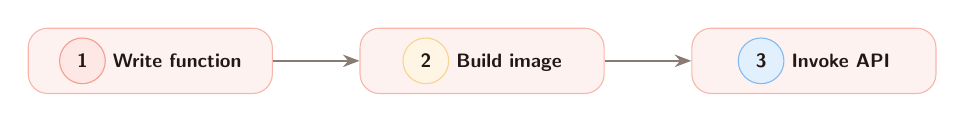
\begin{tikzpicture}[node distance=1.1cm]
  \node[action,minimum width=3.1cm] (write) {\icon{Coral}{1} Write function};
  \node[action,minimum width=3.1cm,right=of write] (build) {\icon{Gold}{2} Build image};
  \node[action,minimum width=3.1cm,right=of build] (call) {\icon{Blue}{3} Invoke API};
  \draw[arr] (write) -- (build);
  \draw[arr] (build) -- (call);
\end{tikzpicture}
\vspace{0.6cm}

{\fontsize{17}{21}\selectfont Users bring Python code. The platform handles execution.}
\end{slideframe}

\begin{slideframe}{Why this project}
\begin{minipage}{7.2cm}
{\fontsize{16}{21}\selectfont
\plainitem{No manual server setup}
\plainitem{Repeatable function builds}
\plainitem{API calls for execution}
\plainitem{Results and artifacts tracked}
}
\end{minipage}
\hfill
\begin{minipage}{5.5cm}
\centering
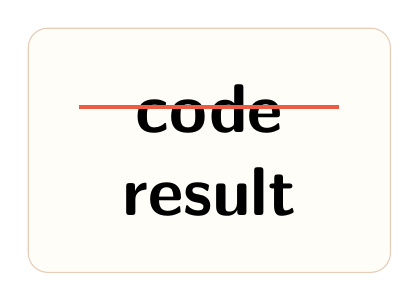
\begin{tikzpicture}
  \node[box,minimum width=4.6cm,minimum height=3.1cm] (b) {};
  \node[font=\fontsize{28}{30}\selectfont\bfseries,align=center] at (b.center) {code\\result};
  \draw[Coral,line width=1.2pt] ([xshift=-1.65cm,yshift=0.55cm]b.center) -- ([xshift=1.65cm,yshift=0.55cm]b.center);
\end{tikzpicture}
\end{minipage}
\end{slideframe}

\begin{slideframe}{Workloads}
\centering
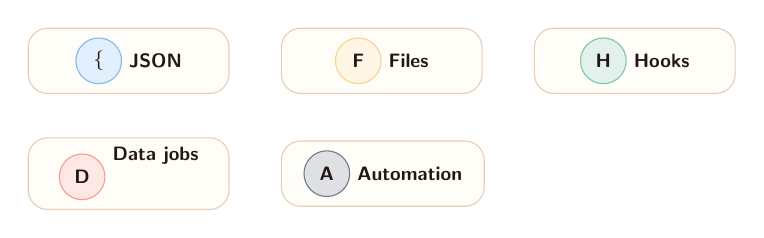
\begin{tikzpicture}[node distance=0.55cm and 0.65cm]
  \node[box,minimum width=2.55cm] (json) {\icon{Blue}{\{} JSON};
  \node[box,minimum width=2.55cm,right=of json] (files) {\icon{Gold}{F} Files};
  \node[box,minimum width=2.55cm,right=of files] (hooks) {\icon{Green}{H} Hooks};
  \node[box,minimum width=2.55cm,below=of json] (data) {\icon{Coral}{D} Data jobs};
  \node[box,minimum width=2.55cm,right=of data] (auto) {\icon{Navy}{A} Automation};
\end{tikzpicture}
\vspace{0.55cm}

{\fontsize{16}{20}\selectfont The prototype targets small Python services and short jobs.}
\end{slideframe}

\begin{slideframe}{Function code}
\begin{minipage}{8.1cm}
\begin{lstlisting}[language=Python]
def main(event, context):
    name = event.get("name", "world")
    print(f"hello {name}")
    return {"message": f"Hello, {name}!"}
\end{lstlisting}
\end{minipage}
\hfill
\begin{minipage}{4.8cm}
{\fontsize{15}{20}\selectfont
\plainitem{\texttt{event} carries input}
\plainitem{\texttt{context} carries metadata}
\plainitem{return value becomes JSON}
}
\end{minipage}
\end{slideframe}

\begin{slideframe}{Dependencies}
\centering
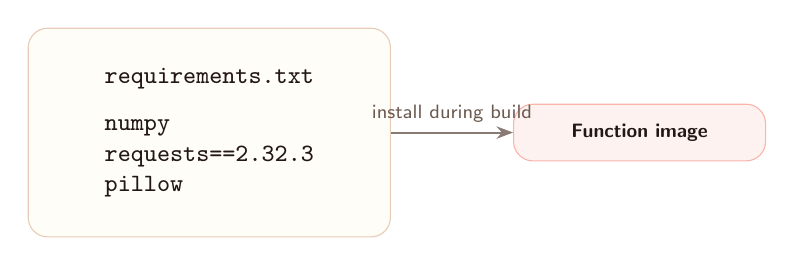
\begin{tikzpicture}
  \node[box,minimum width=4.6cm,minimum height=2.65cm,align=left,font=\ttfamily\small] (req) {
    requirements.txt\\[0.22cm]
    numpy\\
    requests==2.32.3\\
    pillow
  };
  \node[action,minimum width=3.2cm,right=1.55cm of req] (img) {Function image};
  \draw[arr] (req) -- node[above,font=\scriptsize\color{Muted}]{install during build} (img);
\end{tikzpicture}
\end{slideframe}

\begin{slideframe}{Function contract}
\begin{minipage}{6.4cm}
{\fontsize{16}{21}\selectfont
\plainitem{Access mode}
\plainitem{Input file rules}
\plainitem{Expected output names}
}
\end{minipage}
\hfill
\begin{minipage}{6.4cm}
{\fontsize{16}{21}\selectfont
\plainitem{Memory limit}
\plainitem{Function timeout}
\plainitem{Output size limits}
}
\end{minipage}
\vspace{0.55cm}

{\fontsize{15}{20}\selectfont The contract gives callers a predictable API and gives workers clear boundaries.}
\end{slideframe}

\begin{slideframe}{Access modes}
\centering
\renewcommand{\arraystretch}{1.55}
\begin{tabular}{>{\bfseries}p{3.2cm}p{8.5cm}}
\toprule
Private & owner or admin JWT required \\
Token & caller sends a function invocation token \\
Public & caller can invoke without auth \\
\bottomrule
\end{tabular}
\vspace{0.55cm}

{\fontsize{15}{19}\selectfont Invocation tokens stay separate from login JWTs.}
\end{slideframe}

\begin{slideframe}{Synchronous invocation}
\begin{minipage}{6.0cm}
{\fontsize{15}{20}\selectfont
\plainitem{JSON-only functions}
\plainitem{No input files}
\plainitem{No declared output files}
\plainitem{Direct result when fast enough}
}
\end{minipage}
\hfill
\begin{minipage}{7.1cm}
\begin{lstlisting}[language={},basicstyle=\ttfamily\scriptsize]
POST /api/functions/4/invoke-sync/

{"name": "Ada"}

200 OK
{"message": "Hello, Ada!"}
\end{lstlisting}
\end{minipage}
\end{slideframe}

\begin{slideframe}{Asynchronous invocation}
\begin{minipage}{6.0cm}
{\fontsize{15}{20}\selectfont
\plainitem{Durable job path}
\plainitem{Supports files}
\plainitem{Supports polling}
\plainitem{Supports ZIP download}
}
\end{minipage}
\hfill
\begin{minipage}{7.1cm}
\begin{lstlisting}[language={},basicstyle=\ttfamily\scriptsize]
202 Accepted
{
  "invocation_id": 9274,
  "status": "queued",
  "read_token": "inv_..."
}
\end{lstlisting}
\end{minipage}
\end{slideframe}

\begin{slideframe}{Result view}
\centering
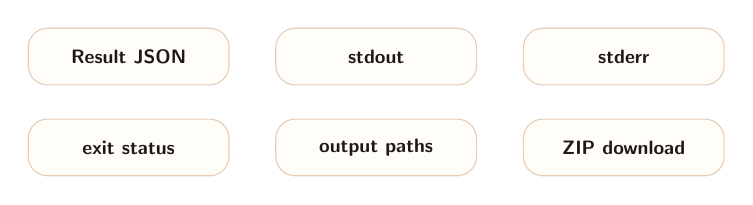
\begin{tikzpicture}[node distance=0.42cm and 0.58cm]
  \node[box,minimum width=2.55cm] (r) {Result JSON};
  \node[box,minimum width=2.55cm,right=of r] (out) {stdout};
  \node[box,minimum width=2.55cm,right=of out] (err) {stderr};
  \node[box,minimum width=2.55cm,below=of r] (exit) {exit status};
  \node[box,minimum width=2.55cm,right=of exit] (files) {output paths};
  \node[box,minimum width=2.55cm,right=of files] (zip) {ZIP download};
\end{tikzpicture}
\vspace{0.55cm}

{\fontsize{15}{19}\selectfont Simple responses stay small. Advanced responses expose diagnostics.}
\end{slideframe}

\begin{slideframe}{Frontend workflow}
\centering
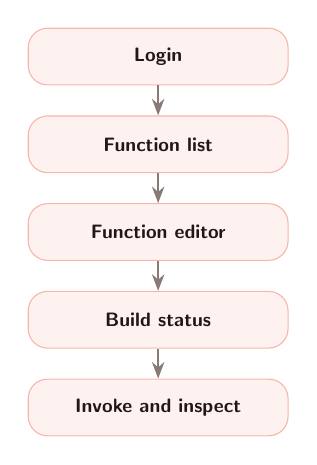
\begin{tikzpicture}[node distance=0.38cm]
  \node[action,minimum width=3.3cm] (login) {Login};
  \node[action,minimum width=3.3cm,below=of login] (list) {Function list};
  \node[action,minimum width=3.3cm,below=of list] (edit) {Function editor};
  \node[action,minimum width=3.3cm,below=of edit] (build) {Build status};
  \node[action,minimum width=3.3cm,below=of build] (invoke) {Invoke and inspect};
  \draw[arr] (login) -- (list);
  \draw[arr] (list) -- (edit);
  \draw[arr] (edit) -- (build);
  \draw[arr] (build) -- (invoke);
\end{tikzpicture}
\end{slideframe}

\begin{slideframe}{Main services}
\centering
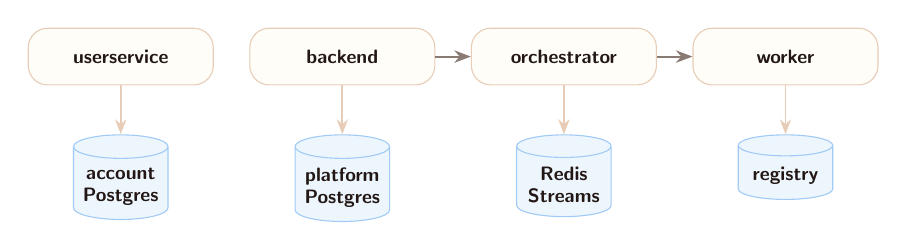
\begin{tikzpicture}[node distance=0.58cm and 0.45cm]
  \node[box,minimum width=2.35cm] (us) {userservice};
  \node[box,minimum width=2.35cm,right=of us] (be) {backend};
  \node[box,minimum width=2.35cm,right=of be] (or) {orchestrator};
  \node[box,minimum width=2.35cm,right=of or] (wo) {worker};
  \node[store,below=0.62cm of us] (upg) {account\\Postgres};
  \node[store,below=0.62cm of be] (pg) {platform\\Postgres};
  \node[store,below=0.62cm of or] (redis) {Redis\\Streams};
  \node[store,below=0.62cm of wo] (reg) {registry};
  \draw[softarr] (us) -- (upg);
  \draw[softarr] (be) -- (pg);
  \draw[softarr] (or) -- (redis);
  \draw[softarr] (wo) -- (reg);
  \draw[arr] (be) -- (or);
  \draw[arr] (or) -- (wo);
\end{tikzpicture}
\end{slideframe}

\begin{slideframe}{Current deployment}
\centering
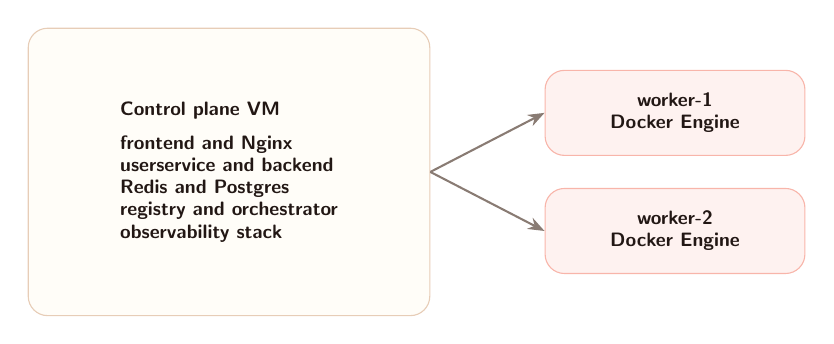
\begin{tikzpicture}[node distance=0.75cm]
  \node[box,minimum width=5.1cm,minimum height=3.65cm,align=left] (cp) {
    \textbf{Control plane VM}\\[0.15cm]
    frontend and Nginx\\
    userservice and backend\\
    Redis and Postgres\\
    registry and orchestrator\\
    observability stack
  };
  \node[action,minimum width=3.3cm,minimum height=1.08cm,right=1.45cm of cp,yshift=0.75cm] (w1) {worker-1\\Docker Engine};
  \node[action,minimum width=3.3cm,minimum height=1.08cm,right=1.45cm of cp,yshift=-0.75cm] (w2) {worker-2\\Docker Engine};
  \draw[arr] (cp.east) -- (w1.west);
  \draw[arr] (cp.east) -- (w2.west);
\end{tikzpicture}
\end{slideframe}

\begin{slideframe}{Build flow}
\centering
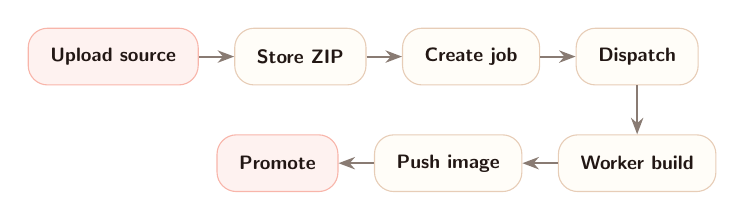
\begin{tikzpicture}[node distance=0.45cm]
  \node[action] (a) {Upload source};
  \node[box,right=of a] (b) {Store ZIP};
  \node[box,right=of b] (c) {Create job};
  \node[box,right=of c] (d) {Dispatch};
  \node[box,below=0.62cm of d] (e) {Worker build};
  \node[box,left=of e] (f) {Push image};
  \node[action,left=of f] (g) {Promote};
  \draw[arr] (a) -- (b);
  \draw[arr] (b) -- (c);
  \draw[arr] (c) -- (d);
  \draw[arr] (d) -- (e);
  \draw[arr] (e) -- (f);
  \draw[arr] (f) -- (g);
\end{tikzpicture}
\end{slideframe}

\begin{slideframe}{Safe rebuilds}
\centering

\begin{tikzpicture}[node distance=0.95cm]
  \node[box,minimum width=3.25cm] (old) {Active image};
  \node[action,minimum width=3.25cm,right=of old] (cand) {Candidate image};
  \node[box,minimum width=3.25cm,right=of cand] (next) {New active image};
  \draw[arr] (old) -- node[above,font=\scriptsize\color{Muted}]{kept live} (cand);
  \draw[arr] (cand) -- node[above,font=\scriptsize\color{Muted}]{promote after success} (next);
\end{tikzpicture}
\vspace{0.65cm}

{\fontsize{15}{19}\selectfont Failed builds do not break the currently callable function.}
\end{slideframe}

\begin{slideframe}{Invocation flow}
\centering
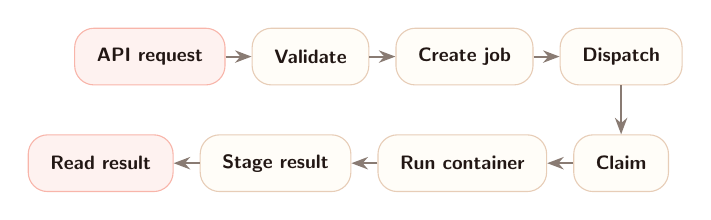
\begin{tikzpicture}[node distance=0.40cm and 0.33cm]
  \node[action] (a) {API request};
  \node[box,right=of a] (b) {Validate};
  \node[box,right=of b] (c) {Create job};
  \node[box,right=of c] (d) {Dispatch};
  \node[box,below=0.62cm of d] (e) {Claim};
  \node[box,left=of e] (f) {Run container};
  \node[box,left=of f] (g) {Stage result};
  \node[action,left=of g] (h) {Read result};
  \draw[arr] (a) -- (b);
  \draw[arr] (b) -- (c);
  \draw[arr] (c) -- (d);
  \draw[arr] (d) -- (e);
  \draw[arr] (e) -- (f);
  \draw[arr] (f) -- (g);
  \draw[arr] (g) -- (h);
\end{tikzpicture}
\end{slideframe}

\begin{slideframe}{Files}
{\fontsize{16}{21}\selectfont
\plainitem{Input files are validated before execution}
\plainitem{Output filenames must be declared during setup}
\plainitem{Unexpected output files are rejected}
\plainitem{Inputs, outputs, and logs expire with the invocation}
}
\end{slideframe}

\begin{slideframe}{Staged artifacts}
\begin{minipage}{6.4cm}
\labeltext{Problem}
{\fontsize{18}{23}\selectfont A file can upload before the job is finalized.}
\end{minipage}
\hfill
\begin{minipage}{6.4cm}
\labeltext{Solution}
{\fontsize{18}{23}\selectfont Hide staged files until the finalizer commits them.}
\end{minipage}
\vspace{0.6cm}
\centering
\pill{Gold}{STAGED}\hspace{0.35cm}
\pill{Green}{COMMITTED}\hspace{0.35cm}
\pill{Blue}{VISIBLE}
\end{slideframe}

\begin{slideframe}{Orchestrator role}
\centering
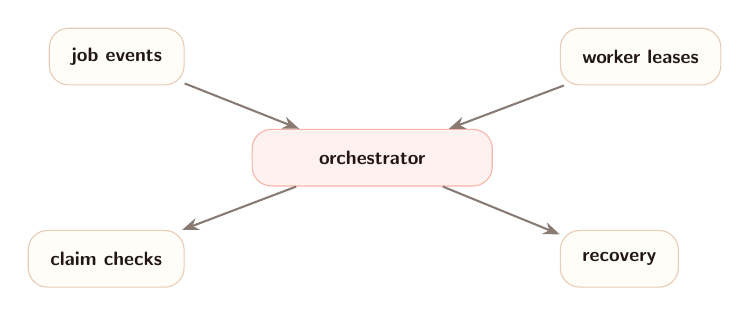
\begin{tikzpicture}[node distance=0.55cm and 0.85cm]
  \node[action,minimum width=3.05cm] (orch) {orchestrator};
  \node[box,above left=of orch] (events) {job events};
  \node[box,above right=of orch] (workers) {worker leases};
  \node[box,below left=of orch] (claims) {claim checks};
  \node[box,below right=of orch] (recovery) {recovery};
  \draw[arr] (events) -- (orch);
  \draw[arr] (workers) -- (orch);
  \draw[arr] (orch) -- (claims);
  \draw[arr] (orch) -- (recovery);
\end{tikzpicture}
\vspace{0.35cm}

{\fontsize{15}{19}\selectfont The orchestrator owns active V2 job state in Redis.}
\end{slideframe}

\begin{slideframe}{Worker role}
{\fontsize{16}{21}\selectfont
\plainitem{Read assigned Redis Stream}
\plainitem{Claim job through the orchestrator}
\plainitem{Download source or inputs from backend}
\plainitem{Run Docker build or function execution}
\plainitem{Report completion and maintain warm containers}
}
\end{slideframe}

\begin{slideframe}{Reliability model}
\centering
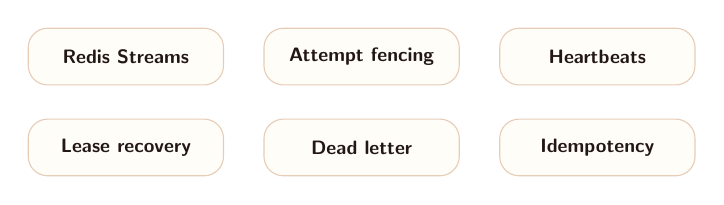
\begin{tikzpicture}[node distance=0.42cm and 0.50cm]
  \node[box,minimum width=2.48cm] (s) {Redis Streams};
  \node[box,minimum width=2.48cm,right=of s] (a) {Attempt fencing};
  \node[box,minimum width=2.48cm,right=of a] (h) {Heartbeats};
  \node[box,minimum width=2.48cm,below=of s] (l) {Lease recovery};
  \node[box,minimum width=2.48cm,right=of l] (d) {Dead letter};
  \node[box,minimum width=2.48cm,right=of d] (i) {Idempotency};
\end{tikzpicture}
\vspace{0.55cm}

{\fontsize{15}{19}\selectfont Jobs either finish, recover, or move to a terminal failure state.}
\end{slideframe}

\begin{slideframe}{Warm containers}
\centering
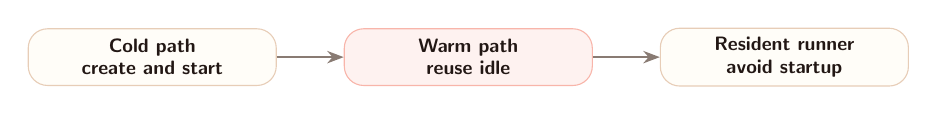
\begin{tikzpicture}[node distance=0.85cm]
  \node[box,minimum width=3.15cm] (cold) {Cold path\\create and start};
  \node[action,minimum width=3.15cm,right=of cold] (warm) {Warm path\\reuse idle};
  \node[box,minimum width=3.15cm,right=of warm] (runner) {Resident runner\\avoid startup};
  \draw[arr] (cold) -- (warm);
  \draw[arr] (warm) -- (runner);
\end{tikzpicture}
\vspace{0.62cm}

\begin{minipage}{5.2cm}
{\fontsize{27}{29}\selectfont\bfseries 3918 ms\par}
{\small\color{Muted}old warm no-op median}
\end{minipage}
\hspace{0.5cm}
\begin{minipage}{5.2cm}
{\fontsize{27}{29}\selectfont\bfseries 88 ms\par}
{\small\color{Muted}resident runner no-op median}
\end{minipage}
\end{slideframe}

\begin{slideframe}{Performance bottlenecks}
{\fontsize{16}{21}\selectfont
\plainitem{Docker container create and start}
\plainitem{Python module imports}
\plainitem{File copying and output handling}
\plainitem{Docker contention during concurrent bursts}
}
\end{slideframe}

\begin{slideframe}{Observability}
\centering
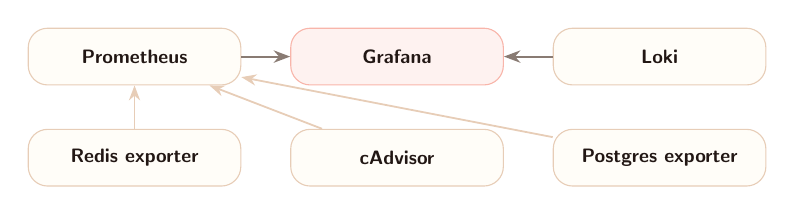
\begin{tikzpicture}[node distance=0.55cm and 0.62cm]
  \node[action,minimum width=2.7cm] (g) {Grafana};
  \node[box,minimum width=2.7cm,left=of g] (p) {Prometheus};
  \node[box,minimum width=2.7cm,right=of g] (l) {Loki};
  \node[box,minimum width=2.7cm,below=of p] (r) {Redis exporter};
  \node[box,minimum width=2.7cm,below=of g] (c) {cAdvisor};
  \node[box,minimum width=2.7cm,below=of l] (pg) {Postgres exporter};
  \draw[arr] (p) -- (g);
  \draw[arr] (l) -- (g);
  \draw[softarr] (r) -- (p);
  \draw[softarr] (c) -- (p);
  \draw[softarr] (pg) -- (p);
\end{tikzpicture}
\end{slideframe}

\begin{slideframe}{Lessons from failures}
{\fontsize{15.5}{20}\selectfont
\plainitem{Backend-centered coordination became too heavy}
\plainitem{Docker copy and export paths were expensive}
\plainitem{Vite dev serving is weak for production}
\plainitem{Worker health missed consume-loop failure}
\plainitem{Private registry refs broke after network changes}
}
\end{slideframe}

\begin{slideframe}{Current state}
\begin{minipage}{6.45cm}
{\fontsize{15.5}{20}\selectfont
\plainitem{Working frontend}
\plainitem{Separate userservice}
\plainitem{V2 orchestrator}
\plainitem{Two distributed workers}
}
\end{minipage}
\hfill
\begin{minipage}{6.45cm}
{\fontsize{15.5}{20}\selectfont
\plainitem{Token invocation}
\plainitem{Warm containers}
\plainitem{Artifact storage}
\plainitem{OpenAPI docs}
}
\end{minipage}
\end{slideframe}

\ifnum\value{slideno}>0\newpage\fi
\begin{tikzpicture}[remember picture,overlay]
  \node[anchor=east,opacity=0.93] at ([xshift=0.65cm]current page.east)
    {
\includegraphics[height=7.2cm]{assets/fleeting-circus-mascot.png}};
  \fill[Coral] ([xshift=0.75cm,yshift=-0.65cm]current page.north west) circle (0.09cm);
  \fill[Gold] ([xshift=1.05cm,yshift=-0.65cm]current page.north west) circle (0.06cm);
\end{tikzpicture}
\vspace*{1.05cm}
\hspace*{0.9cm}
\begin{minipage}{8.0cm}
  \raggedright
  \labeltext{Next work}
  \vspace{0.2cm}
  {\fontsize{27}{31}\selectfont\bfseries Reliability and\\production hardening\par}
  \vspace{0.45cm}
  {\fontsize{13.5}{17}\selectfont
  \plainitem{Recover worker consume-loop failures}
  \plainitem{Harden worker and control plane networking}
  \plainitem{Add stronger build resource limits}
  \plainitem{Serve static frontend files}
  \plainitem{Run longer failure and load tests}
  }
\end{minipage}

\end{document}
